\documentclass[../main.tex]{subfiles}
\graphicspath{{\subfix{../images/}}}
\begin{document}
\label{Ex:headstand}
\index{exercises!handstand}

\noindent
\begin{tabular}{p{5.4cm} p{6.5cm}}
  \raisebox{-\totalheight}{  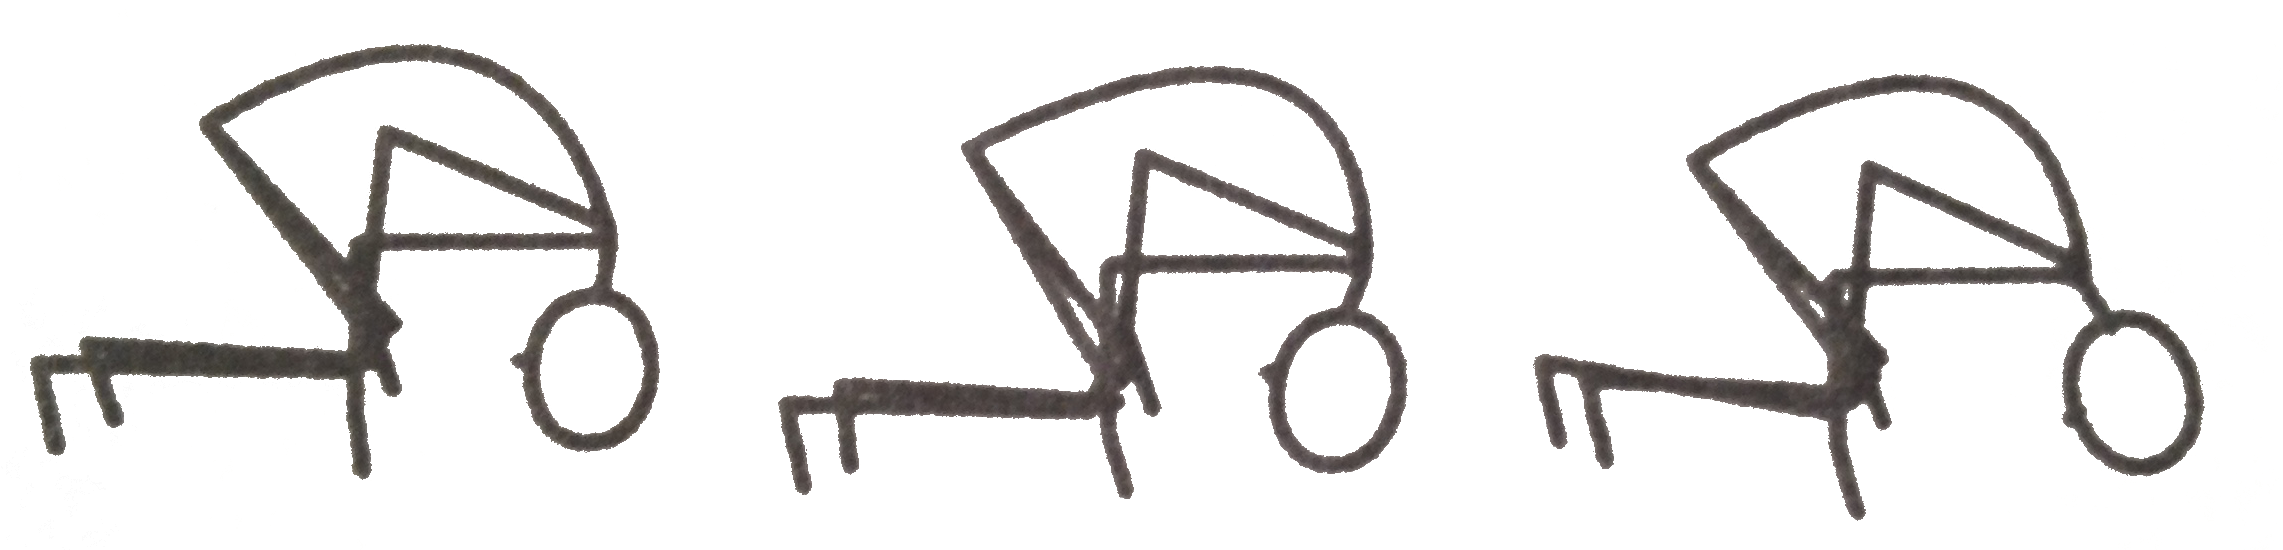
\includegraphics[width=5.4cm]{HS_position} }\label{sf:headstand}
&
{Kneel} down with your toes flexed up and make a {triangle with your hands and the head},
by putting the crown (the highest point) on the ground.

                                                                            

{Roll your head very gently} back and forwards.

\hspace{6cm}\\
    \raisebox{-\totalheight}{  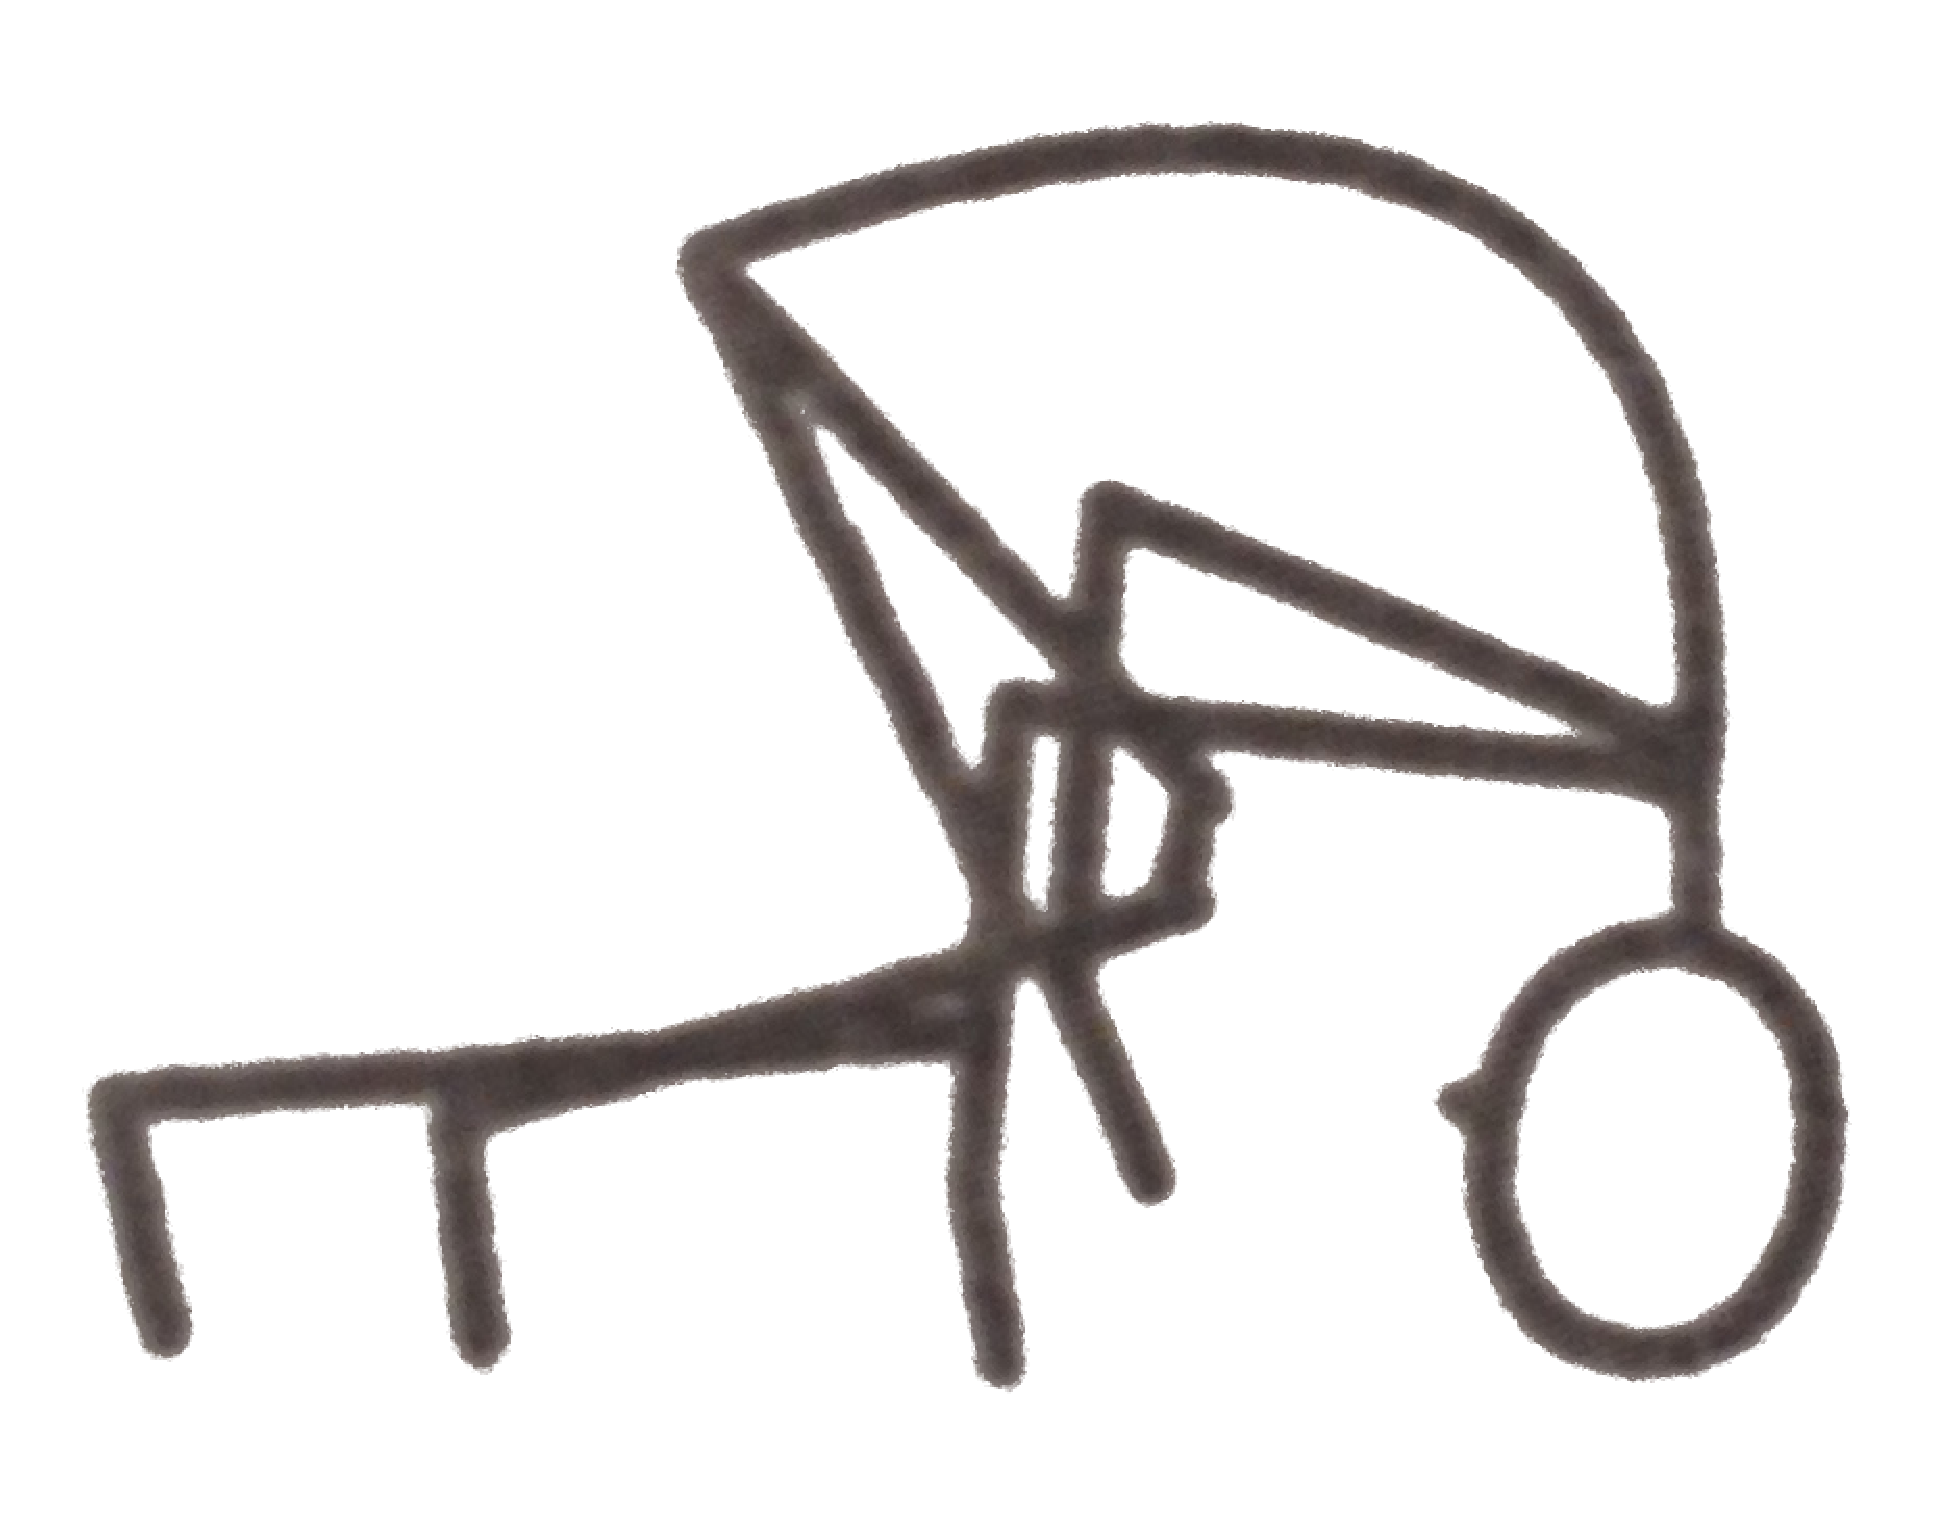
\includegraphics[width=1.7cm]{HS_lift} } &
{Lift your knees} a bit off the ground. The pressure on the crown increases.
Try again in this position to {roll} a bit forward and backwards. This will be way more difficult.

\hspace{8cm}\\
    \raisebox{-\totalheight}{  \includegraphics[width=5cm]{HS_upwards} } &
  {Walk} with your {feet} closer towards your head and push your {backside towards the ceiling}.

Try to bring your feet away from the ground by making a ``hollow back''.

It's important to {first bring the feet up}, not the  legs.   

\hspace{2cm}\\
  \raisebox{-0.6\totalheight}{  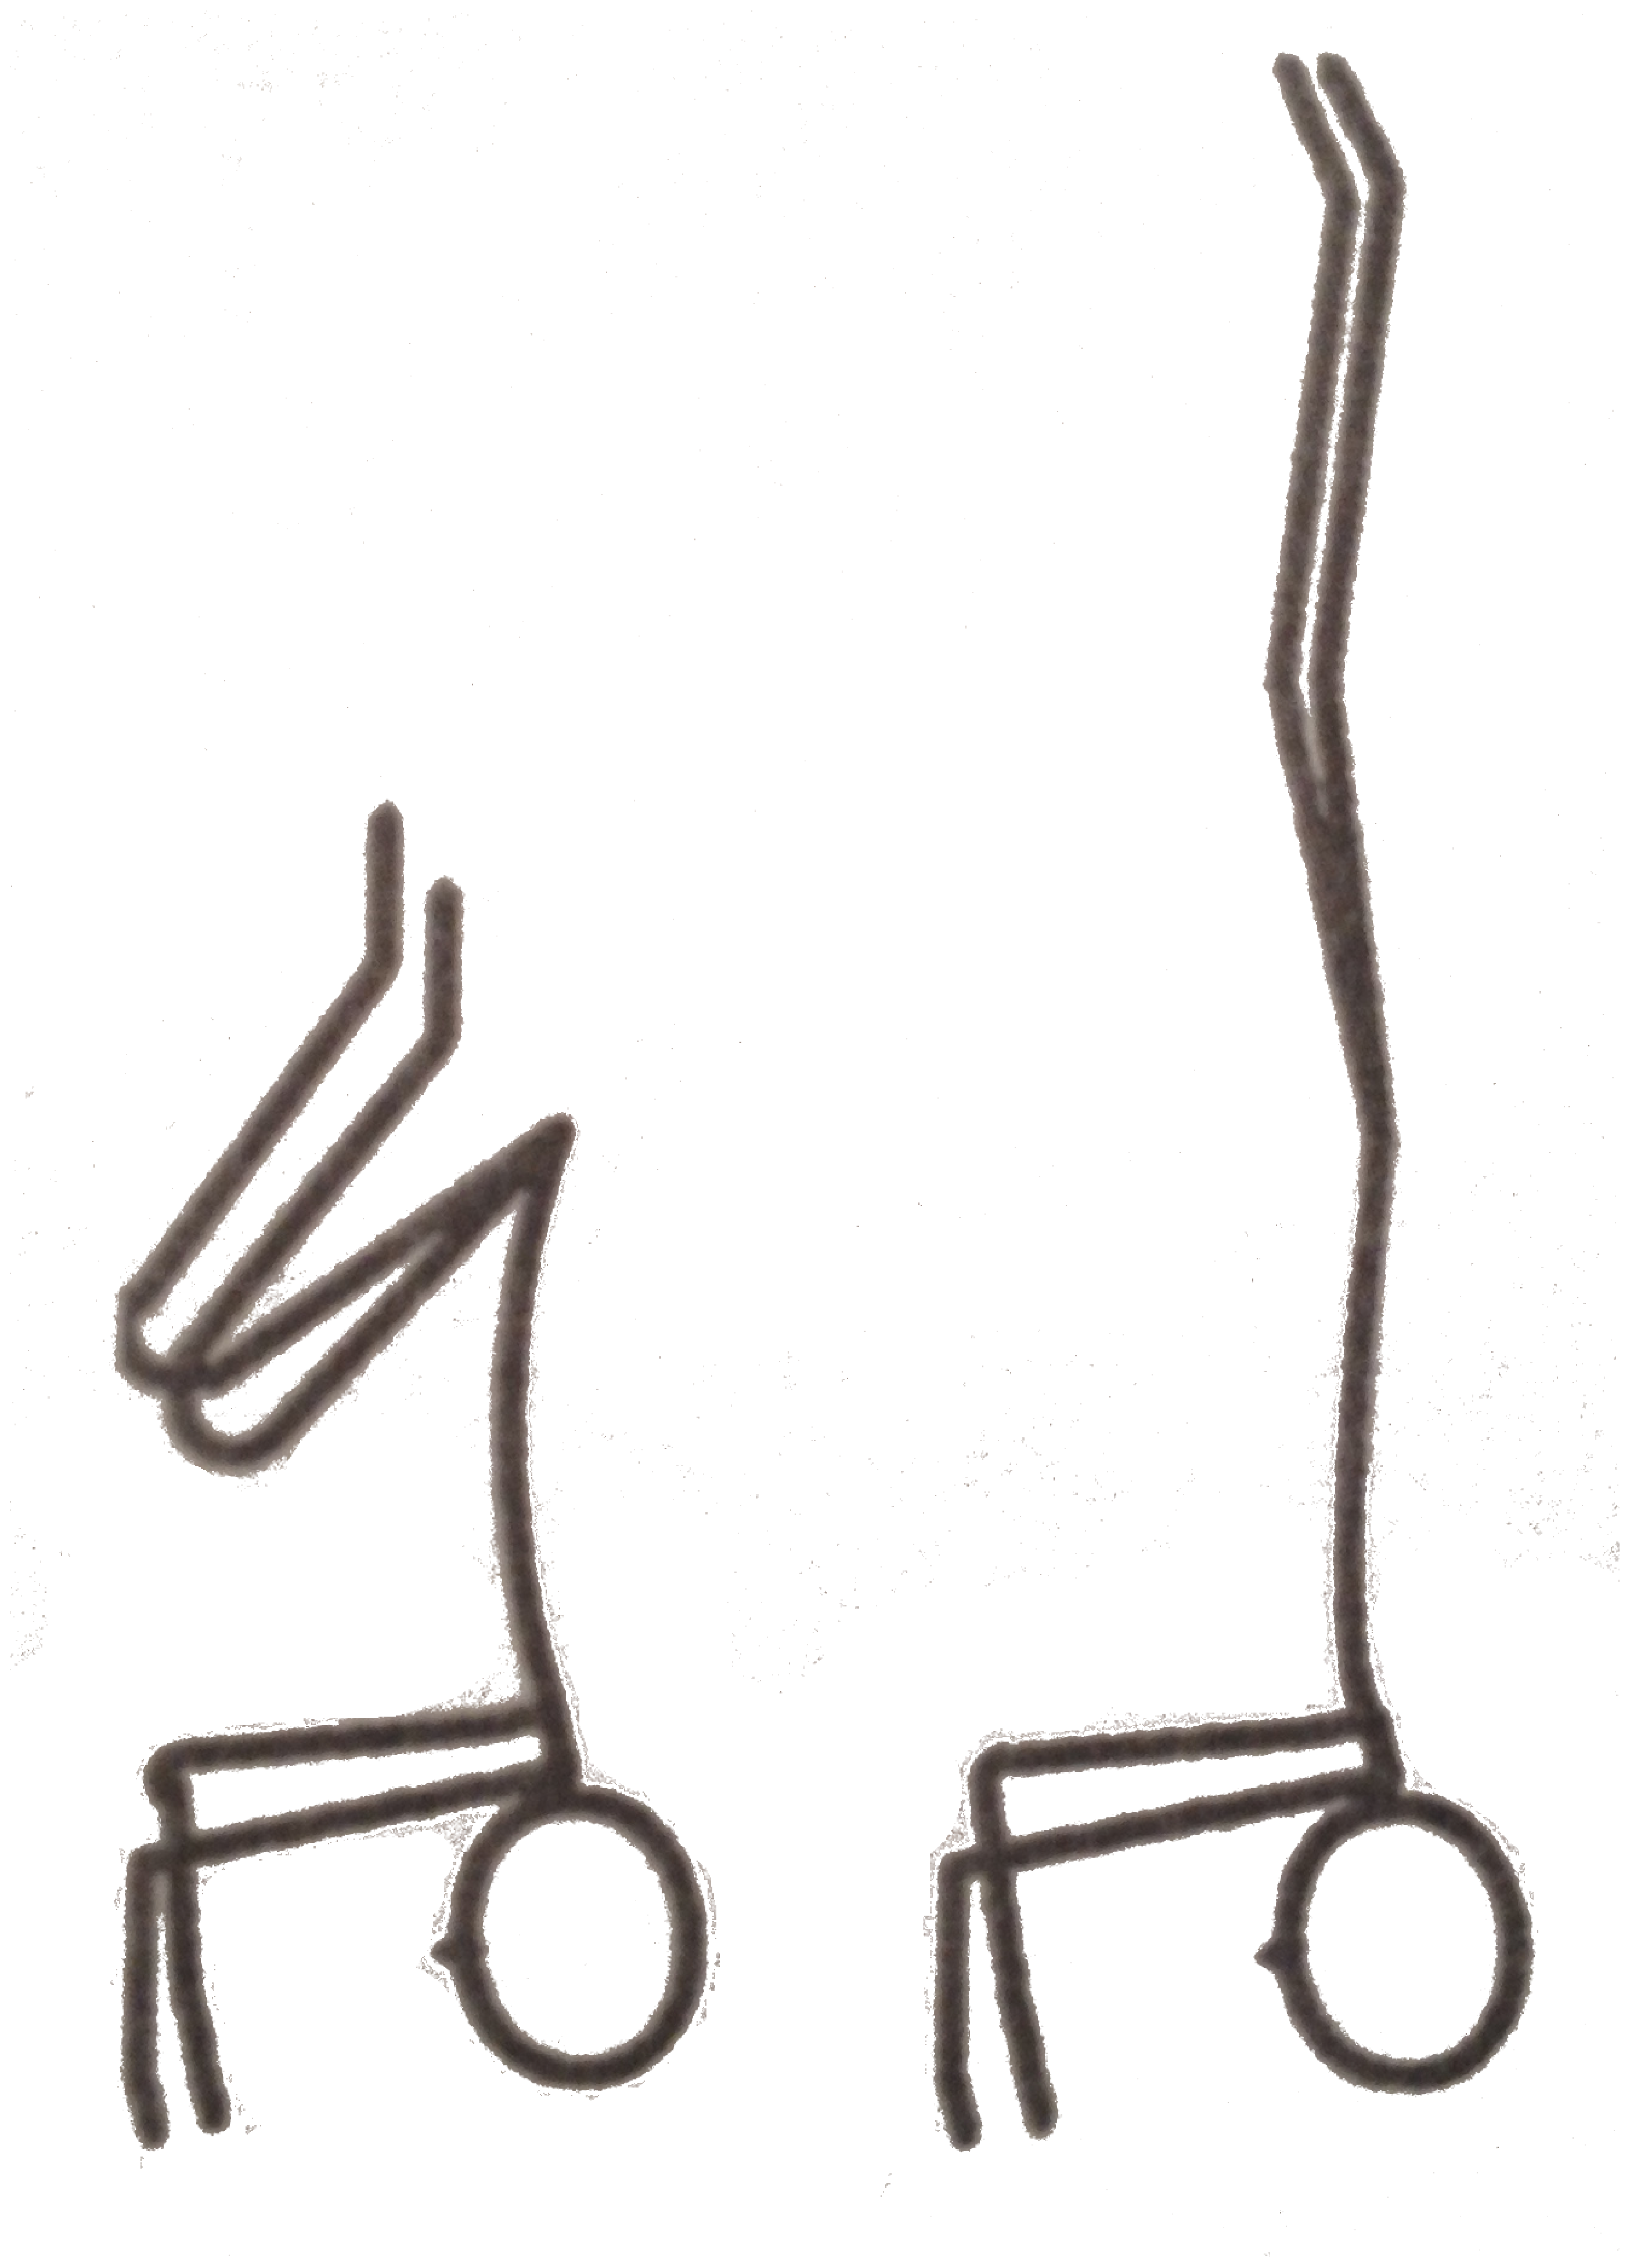
\includegraphics[width=2.4cm]{HS_Up} }
  & Now ``pull'' your {legs slowly up} with your hips.
    Let them {first be tucked in} and only then {slowly up} when you feel safe to do so.
\end{tabular}
\newpage

\end{document}